% 这是中国科学院大学计算机科学与技术专业《计算机组成原理（研讨课）》使用的实验报告 Latex 模板
% 本模板与 2024 年 2 月 Jun-xiong Ji 完成, 更改自由 Shing-Ho Lin 和 Jun-Xiong Ji 于 2022 年 9 月共同完成的基础物理实验模板
% 如有任何问题, 请联系: jijunxoing21@mails.ucas.ac.cn
% This is the LaTeX template for report of Experiment of Computer Organization and Design courses, based on its provided Word template. 
% This template is completed on Febrary 2024, based on the joint collabration of Shing-Ho Lin and Junxiong Ji in September 2022. 
% Adding numerous pictures and equations leads to unsatisfying experience in Word. Therefore LaTeX is better. 
% Feel free to contact me via: jijunxoing21@mails.ucas.ac.cn

\documentclass[11pt]{article}

\usepackage[a4paper]{geometry}
\geometry{left=2.0cm,right=2.0cm,top=2.5cm,bottom=2.5cm}

\usepackage{ctex} % 支持中文的LaTeX宏包
\usepackage{amsmath,amsfonts,graphicx,subfigure,amssymb,bm,amsthm,mathrsfs,mathtools,breqn} % 数学公式和符号的宏包集合
\usepackage{algorithm,algorithmicx} % 算法和伪代码
\usepackage[noend]{algpseudocode} % 算法和伪代码
\usepackage{fancyhdr} % 自定义页眉页脚
\usepackage[framemethod=TikZ]{mdframed} % 创建带边框的框架
\usepackage{fontspec} % 字体设置
\usepackage{adjustbox} % 调整盒子大小
\usepackage{fontsize} % 设置字体大小
\usepackage{tikz,xcolor} % 绘制图形和使用颜色
\usepackage{multicol} % 多栏排版
\usepackage{multirow} % 表格中合并单元格
\usepackage{pdfpages} % 插入PDF文件
\usepackage{listings} % 在文档中插入源代码
\usepackage{wrapfig} % 文字绕排图片
\usepackage{bigstrut,multirow,rotating} % 支持在表格中使用特殊命令
\usepackage{booktabs} % 创建美观的表格
\usepackage{circuitikz} % 绘制电路图
\usepackage{zhnumber} % 中文序号（用于标题）
\usepackage{tabularx} % 表格折行
\usepackage{tikz}
\usetikzlibrary{positioning} % 加载 positioning 库

\definecolor{dkgreen}{rgb}{0,0.6,0}
\definecolor{gray}{rgb}{0.5,0.5,0.5}
\definecolor{mauve}{rgb}{0.58,0,0.82}
\lstset{
  frame=tb,
  aboveskip=3mm,
  belowskip=3mm,
  showstringspaces=false,
  columns=flexible,
  framerule=1pt,
  rulecolor=\color{gray!35},
  backgroundcolor=\color{gray!5},
  basicstyle={\small\ttfamily},
  numbers=none,
  numberstyle=\tiny\color{gray},
  keywordstyle=\color{blue},
  commentstyle=\color{dkgreen},
  stringstyle=\color{mauve},
  breaklines=true,
  breakatwhitespace=true,
  tabsize=3,
}

% 超链接支持 (一定要在大多数包之后, cleveref 之前)
% colorlinks=true 使链接文字着色而不是加方框; hidelinks 可去掉颜色
\usepackage[colorlinks=true,linkcolor=blue,citecolor=blue,urlcolor=magenta]{hyperref}

% 轻松引用, 可以用\cref{}指令直接引用, 自动加前缀. 需要在 hyperref 之后加载
% 例: 图片label为fig:1  => \cref{fig:1} -> Figure.1; \ref{fig:1} -> 1 (纯数字)
\usepackage[capitalize]{cleveref}
% \crefname{section}{Sec.}{Secs.}
\Crefname{section}{Section}{Sections}
\Crefname{table}{Table}{Tables}
\crefname{table}{Table.}{Tabs.}

% \setmainfont{Palatino Linotype.ttf}
% \setCJKmainfont{SimHei.ttf}
% \setCJKsansfont{Songti.ttf}
% \setCJKmonofont{SimSun.ttf}
\punctstyle{kaiming}
% 偏好的几个字体, 可以根据需要自行加入字体ttf文件并调用

\renewcommand{\emph}[1]{\begin{kaishu}#1\end{kaishu}}

% 对 section 等环境的序号使用中文
\renewcommand \thesection{\zhnum{section}、}
\renewcommand \thesubsection{\arabic{section}.\arabic{subsection}}

\tikzset{
    link/.style={draw, thick, -stealth} % 定义 link 样式，包含绘制、粗线条和箭头
}


%%%%%%%%%%%%%%%%%%%%%%%%%%%
%改这里可以修改实验报告表头的信息
\newcommand{\name}{寇逸欣}
\newcommand{\studentNum}{2023K8009922004}
\newcommand{\major}{计算机科学与技术}
\newcommand{\labNum}{05}
\newcommand{\labName}{生成树机制实验}
%%%%%%%%%%%%%%%%%%%%%%%%%%%

\begin{document}

\input{tex_file/head.tex}

\section{实验内容}

本实验主要包括以下内容：
\begin{enumerate}
	\item 基于已有代码，实现生成树运行机制，对于给定拓扑(four_node_ring.py)，计算输出相应状态下的最小生成树拓扑
	\item 自己构造一个不少于7个节点，冗余链路不少于2条的拓扑，节点和端口的命名规则可参考four_node_ring.py，使用stp程序计算输出最小生成树拓扑
\end{enumerate}

\section{实验流程}
本实验需要完成的是stp.c文件中的stp_handle_config_packet函数。这个函数的作用是根据接收到的config包，更新端口的状态，并且重新计算生成树的结构。本次实验是
静态生成树，不用考虑拓扑变动下的生成树重构、如何与交换机转发学习共存以及如何快速构建生成树等问题。

首先，我们需要实现一个函数，用于比较两个config包的优先级，以确定哪个config包更优。比较的规则如下：
\begin{enumerate}
	\item 如果两者认为的根节点ID不同，则根节点ID小的一方优先级高
	\item 如果两者到根节点的开销不同，则开销小的一方优先级高
	\item 如果两者到根节点的上一跳节点不同，则上一跳节点ID小的一方优先级高
	\item 如果两者到根节点的上一跳端口不同，则上一跳端口ID小的一方优先级高
\end{enumerate}

代码实现如下：
\begin{lstlisting}[language=C]
static int stp_tuple_cmp(u64 r1, u32 c1, u64 s1, u16 p1, u64 r2, u32 c2, u64 s2, u16 p2)
{
    if (r1 != r2) return (r1 < r2) ? -1 : 1;
    if (c1 != c2) return (c1 < c2) ? -1 : 1;
    if (s1 != s2) return (s1 < s2) ? -1 : 1;
    if (p1 != p2) return (p1 < p2) ? -1 : 1;
    return 0;
}
\end{lstlisting}

接下来，我们需要实现函数stp_recompute来重新计算生成树的结构。这个函数会遍历所有端口，找出每个节点到根节点的最优路径，并更新端口的状态。代码实现如下：
\begin{lstlisting}[language=C]
static void stp_recompute(stp_t *stp)
{
    // 1) 选根端口：只在“对端更优”的端口中选
    stp_port_t *best_port = NULL;
    u64 best_root = 0;
    u32 best_cost = 0;
    u64 best_sw = 0;
    u16 best_pid = 0;

    for (int i = 0; i < stp->nports; i++) {
        stp_port_t *p = &stp->ports[i];
        if (p->designated_switch == stp->switch_id) continue;

        u64 r = p->designated_root;
        u32 c = p->designated_cost + p->path_cost;
        u64 s = p->designated_switch;
        u16 pid = p->designated_port;

        if (!best_port || stp_tuple_cmp(r, c, s, pid, best_root, best_cost, best_sw, best_pid) < 0) {
            best_port = p;
            best_root = r;
            best_cost = c;
            best_sw = s;
            best_pid = pid;
        }
    }

    // 2) 更新本桥的根信息
    if (!best_port) {
        stp->designated_root = stp->switch_id;
        stp->root_path_cost = 0;
        stp->root_port = NULL;
    } else {
        stp->designated_root = best_root;
        stp->root_path_cost = best_cost;
        stp->root_port = best_port;
    }

    // 3) 刷新各端口的 designated 信息
    for (int i = 0; i < stp->nports; i++) {
        stp_port_t *q = &stp->ports[i];

        if (stp->root_port && q->port_id == stp->root_port->port_id)
            continue;

        u64 my_r = stp->designated_root;
        u32 my_c = stp->root_path_cost;
        u64 my_s = stp->switch_id;
        u16 my_p = q->port_id;

        if (stp_tuple_cmp(my_r, my_c, my_s, my_p,
                          q->designated_root, q->designated_cost,
                          q->designated_switch, q->designated_port) < 0) {
            q->designated_root = my_r;
            q->designated_cost = my_c;
            q->designated_switch = my_s;
            q->designated_port = my_p;
        }
    }
}
\end{lstlisting}

最后，我们利用上面实现的函数，在stp_handle_config_packet函数中处理接收到的config包。代码实现如下：

\begin{lstlisting}[language=C]
static void stp_handle_config_packet(stp_t *stp, stp_port_t *p, struct stp_config *config)
{
    u64 recv_root_id = ntohll(config->root_id);
    u32 recv_root_path_cost = ntohl(config->root_path_cost);
    u64 recv_switch_id = ntohll(config->switch_id);
    u16 recv_port_id = ntohs(config->port_id);

    bool superior = stp_tuple_cmp(
        recv_root_id, recv_root_path_cost, recv_switch_id, recv_port_id,
        p->designated_root, p->designated_cost, p->designated_switch, p->designated_port
    ) < 0;

    if (superior) {
        p->designated_root = recv_root_id;
        p->designated_cost = recv_root_path_cost;
        p->designated_switch = recv_switch_id;
        p->designated_port = recv_port_id;

        stp_recompute(stp);

        stp_send_config(stp);
    } else {
        if (stp_port_is_designated(p)) {
            stp_port_send_config(p);
        }
    }
}
\end{lstlisting}

\section{实验结果及分析}
\subsection{实验结果}
对于四节点环形拓扑(four_node_ring.py)，运行stp程序后，输出的最小生成树拓扑如下：
\begin{lstlisting}
NODE b1 dumps:
INFO: this switch is root.
INFO: port id: 01, role: DESIGNATED.
INFO: 	designated ->root: 0101, ->switch: 0101, ->port: 01, ->cost: 0.
INFO: port id: 02, role: DESIGNATED.
INFO: 	designated ->root: 0101, ->switch: 0101, ->port: 02, ->cost: 0.

NODE b2 dumps:
INFO: non-root switch, designated root: 0101, root path cost: 1.
INFO: port id: 01, role: ROOT.
INFO: 	designated ->root: 0101, ->switch: 0101, ->port: 01, ->cost: 0.
INFO: port id: 02, role: DESIGNATED.
INFO: 	designated ->root: 0101, ->switch: 0201, ->port: 02, ->cost: 1.

NODE b3 dumps:
INFO: non-root switch, designated root: 0101, root path cost: 1.
INFO: port id: 01, role: ROOT.
INFO: 	designated ->root: 0101, ->switch: 0101, ->port: 02, ->cost: 0.
INFO: port id: 02, role: DESIGNATED.
INFO: 	designated ->root: 0101, ->switch: 0301, ->port: 02, ->cost: 1.

NODE b4 dumps:
INFO: non-root switch, designated root: 0101, root path cost: 2.
INFO: port id: 01, role: ROOT.
INFO: 	designated ->root: 0101, ->switch: 0201, ->port: 02, ->cost: 1.
INFO: port id: 02, role: ALTERNATE.
INFO: 	designated ->root: 0101, ->switch: 0301, ->port: 02, ->cost: 1.
\end{lstlisting}

示意图如下：
\begin{figure}[H]
\centering
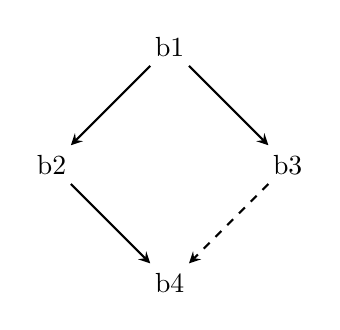
\begin{tikzpicture}
	\node (b1) [switch] at (0,1.5) {b1};
	\node (b2) [switch] at (-1.5,0) {b2};
	\node (b3) [switch] at (1.5,0) {b3};
	\node (b4) [switch] at (0,-1.5) {b4};

	\draw[link] (b1) -- (b2);
	\draw[link] (b1) -- (b3);
	\draw[link] (b2) -- (b4);
	\draw[link, dashed] (b3) -- (b4);
\end{tikzpicture}
\caption{四节点环形拓扑的最小生成树}
\label{fig:four_node_ring}
\end{figure}

八节点拓扑(my_topology.py)，运行stp程序后，输出的最小生成树拓扑如下：
\begin{lstlisting}
NODE b1 dumps:
INFO: this switch is root.
INFO: port id: 01, role: DESIGNATED.
INFO: 	designated ->root: 0101, ->switch: 0101, ->port: 01, ->cost: 0.
INFO: port id: 02, role: DESIGNATED.
INFO: 	designated ->root: 0101, ->switch: 0101, ->port: 02, ->cost: 0.
INFO: port id: 03, role: DESIGNATED.
INFO: 	designated ->root: 0101, ->switch: 0101, ->port: 03, ->cost: 0.

NODE b2 dumps:
INFO: non-root switch, designated root: 0101, root path cost: 1.
INFO: port id: 01, role: ROOT.
INFO: 	designated ->root: 0101, ->switch: 0101, ->port: 01, ->cost: 0.
INFO: port id: 02, role: DESIGNATED.
INFO: 	designated ->root: 0101, ->switch: 0201, ->port: 02, ->cost: 1.
INFO: port id: 03, role: DESIGNATED.
INFO: 	designated ->root: 0101, ->switch: 0201, ->port: 03, ->cost: 1.

NODE b3 dumps:
INFO: non-root switch, designated root: 0101, root path cost: 1.
INFO: port id: 01, role: ROOT.
INFO: 	designated ->root: 0101, ->switch: 0101, ->port: 02, ->cost: 0.
INFO: port id: 02, role: DESIGNATED.
INFO: 	designated ->root: 0101, ->switch: 0301, ->port: 02, ->cost: 1.
INFO: port id: 03, role: DESIGNATED.
INFO: 	designated ->root: 0101, ->switch: 0301, ->port: 03, ->cost: 1.

NODE b4 dumps:
INFO: non-root switch, designated root: 0101, root path cost: 2.
INFO: port id: 01, role: ROOT.
INFO: 	designated ->root: 0101, ->switch: 0201, ->port: 02, ->cost: 1.
INFO: port id: 02, role: ALTERNATE.
INFO: 	designated ->root: 0101, ->switch: 0301, ->port: 02, ->cost: 1.
INFO: port id: 03, role: DESIGNATED.
INFO: 	designated ->root: 0101, ->switch: 0401, ->port: 03, ->cost: 2.

NODE b5 dumps:
INFO: non-root switch, designated root: 0101, root path cost: 1.
INFO: port id: 01, role: ROOT.
INFO: 	designated ->root: 0101, ->switch: 0101, ->port: 03, ->cost: 0.
INFO: port id: 02, role: DESIGNATED.
INFO: 	designated ->root: 0101, ->switch: 0501, ->port: 02, ->cost: 1.
INFO: port id: 03, role: DESIGNATED.
INFO: 	designated ->root: 0101, ->switch: 0501, ->port: 03, ->cost: 1.

NODE b6 dumps:
INFO: non-root switch, designated root: 0101, root path cost: 2.
INFO: port id: 01, role: ROOT.
INFO: 	designated ->root: 0101, ->switch: 0201, ->port: 03, ->cost: 1.
INFO: port id: 02, role: ALTERNATE.
INFO: 	designated ->root: 0101, ->switch: 0501, ->port: 02, ->cost: 1.
INFO: port id: 03, role: DESIGNATED.
INFO: 	designated ->root: 0101, ->switch: 0601, ->port: 03, ->cost: 2.

NODE b7 dumps:
INFO: non-root switch, designated root: 0101, root path cost: 2.
INFO: port id: 01, role: ROOT.
INFO: 	designated ->root: 0101, ->switch: 0301, ->port: 03, ->cost: 1.
INFO: port id: 02, role: ALTERNATE.
INFO: 	designated ->root: 0101, ->switch: 0501, ->port: 03, ->cost: 1.
INFO: port id: 03, role: DESIGNATED.
INFO: 	designated ->root: 0101, ->switch: 0701, ->port: 03, ->cost: 2.

NODE b8 dumps:
INFO: non-root switch, designated root: 0101, root path cost: 3.
INFO: port id: 01, role: ROOT.
INFO: 	designated ->root: 0101, ->switch: 0401, ->port: 03, ->cost: 2.
INFO: port id: 02, role: ALTERNATE.
INFO: 	designated ->root: 0101, ->switch: 0601, ->port: 03, ->cost: 2.
INFO: port id: 03, role: ALTERNATE.
INFO: 	designated ->root: 0101, ->switch: 0701, ->port: 03, ->cost: 2.
\end{lstlisting}

示意图如下：
\begin{figure}[H]
\centering
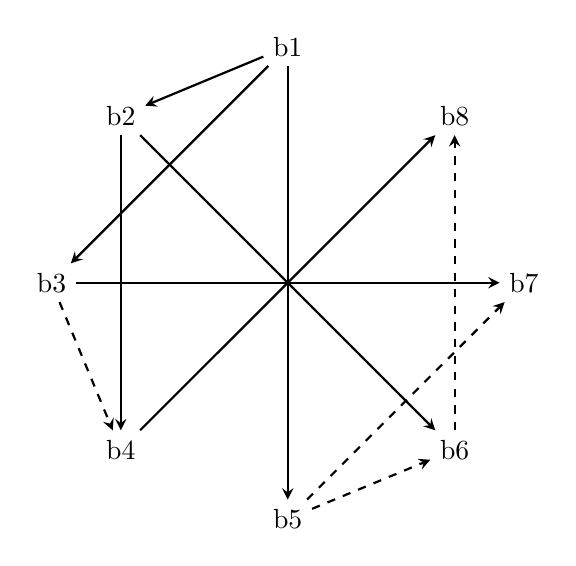
\begin{tikzpicture}
    \node (b1) [switch] at (0, 3) {b1};
    \node (b2) [switch] at (-2.12, 2.12) {b2};
    \node (b3) [switch] at (-3, 0) {b3};
    \node (b4) [switch] at (-2.12, -2.12) {b4};
    \node (b5) [switch] at (0, -3) {b5};
    \node (b6) [switch] at (2.12, -2.12) {b6};
    \node (b7) [switch] at (3, 0) {b7};
    \node (b8) [switch] at (2.12, 2.12) {b8};

    % 活动链路（最小生成树中的链路）- 实线
    \draw[link] (b1) -- (b2); % b2端口01为ROOT
    \draw[link] (b1) -- (b3); % b3端口01为ROOT
    \draw[link] (b1) -- (b5); % b5端口01为ROOT
    \draw[link] (b2) -- (b4); % b4端口01为ROOT
    \draw[link] (b2) -- (b6); % b6端口01为ROOT
    \draw[link] (b3) -- (b7); % b7端口01为ROOT
    \draw[link] (b4) -- (b8); % b8端口01为ROOT

    % 阻塞链路（被STP阻塞的链路）- 虚线
    \draw[link, dashed] (b5) -- (b6); % b6端口02为ALTERNATE
    \draw[link, dashed] (b5) -- (b7); % b7端口02为ALTERNATE
    \draw[link, dashed] (b6) -- (b8); % b8端口02为ALTERNATE
	\draw[link, dashed] (b3) -- (b4); % b4端口02为ALTERNATE
\end{tikzpicture}
\caption{八节点拓扑的最小生成树}
\label{fig:my_topology_corrected}
\end{figure}

\subsection{结果分析}
我们以四节点的环形拓扑为例进行分析。最开始，所有节点都认为自己是根节点，所有端口都被置为指定端口。
当b1发送它的config包时，b2和b3收到后发现b1的根节点ID更小，因此更新了自己的根节点信息，并将连接b1的端口设为根端口。
随后，b2和b3也发送了各自的config包，b4收到后发现通过b2或b3到达b1的路径开销相同，但由于b2的交换机ID更小，因此选择通过b2作为根端口。
最终，b4通过比较收到的config包，确定连接b3的端口为其他端口，从而形成了最小生成树。

\section{DEBUG分析}
在调试过程中，我遇到了一些问题，主要集中在以下几个方面：
\begin{enumerate}
	\item 计算路径开销的时候，错误的多加了端口的路径开销，导致计算结果不正确。通过对比reference生成的正确结果，发现应该只加上收到的config包中的路径开销。
	\item 在比较config包优先级时，忘记考虑上一跳端口的优先级，导致在某些情况下无法正确选择最优路径。通过补充比较逻辑，解决了这个问题。
\end{enumerate}

\end{document}

